\documentclass{article}
\usepackage[a4paper, margin=5em]{geometry}
\usepackage{fancyhdr}
\usepackage{lastpage}
\usepackage{graphicx}
\usepackage{hyperref}
\usepackage{ngerman}
\usepackage{enumitem}
\usepackage{csquotes}
\usepackage{caption}

\newcommand{\gqq}[1]{\glqq{}#1\grqq{}}

\pagestyle{fancy}
\fancyhf{}
\renewcommand{\headrulewidth}{0pt}
\setlength\parindent{0pt}
\fancyfoot{}

\lfoot{}
\cfoot{Seite \thepage\ / \pageref*{LastPage}}
\rfoot{}

\hypersetup{
    colorlinks=true,
    linktoc=all,
    urlcolor=blue
}

\author{Tim Wende}
\date{\today}
\title{\textbf{Hausaufgabe 6}}

\begin{document}
    \maketitle
    \section*{Veranstaltungsverwaltungssystem}

    Gegeben sei folgende Beschreibung für ein Veranstaltungsverwaltungssystem:

    \underline{Personen} haben Zeichenketten als \texttt{Name}.
    \underline{Studierende} sind Personen, erben also die Eigenschaften von Person, haben aber zusätzlich eine ganzzahlige \texttt{Matrikelnummer} und nehmen an beliebig vielen Veranstaltungen teil.
    Eine \underline{Veranstaltung} hat potentiell beliebig viele Teilnehmende, wird aber von einem, zwei oder drei \underline{MitarbeiterInnen} betreut.
    Eine Veranstaltung hat eine \texttt{Veranstaltungsnummer} und einen \texttt{Titel}.
    \underline{Seminare} und \underline{Vorlesungen} sind spezielle Veranstaltungen.
    Ein Seminar hat eine begrenzte \texttt{Anzahl an Plätzen}, für eine Vorlesung wird eine \underline{Klausur} angeboten oder nicht.
    MitarbeiterInnen sind Personen und betreuen eine bis fünf Veranstaltungen und haben eine \texttt{Personalnummer}.
    \underline{ProfessorInnen} und \underline{AssistentInnen} sind Mitarbeitende.
    AssistentInnen sind bei genau einem/r ProfessorIn beschäftigt und haben eine bestimmt \texttt{Finanzierung} (Zeichenkette).
    Ein/e ProfessorIn hat ein \texttt{Lehrgebiet} (Zeichenkette), beschäftigt beliebig viele AssistentInnen und ist InhaberIn von genau einem \underline{Lehrstuhl}.
    Ein Lehrstuhl hat eine \texttt{Bezeichnung} und genau einen/e ProfessorIn als InhaberIn.
    
    Erstellen Sie anhand der obigen Beschreibung ein \textbf{Klassendiagramm}. Ihr Diagramm sollte folgende Punkte beinhalten:
    
    \begin{itemize}
        \setlength{\itemsep}{0em}
        \item \textbf{Generalisierungsbeziehungen},
        \item \textbf{Assoziationen} mit Assoziationsnamen und Leserichtung,
        \item \textbf{Multiplizitäten} sowie
        \item \textbf{Attributnamen} und (sinnvolle) \textbf{–typen}.
    \end{itemize}

    \begin{figure}[ht]
        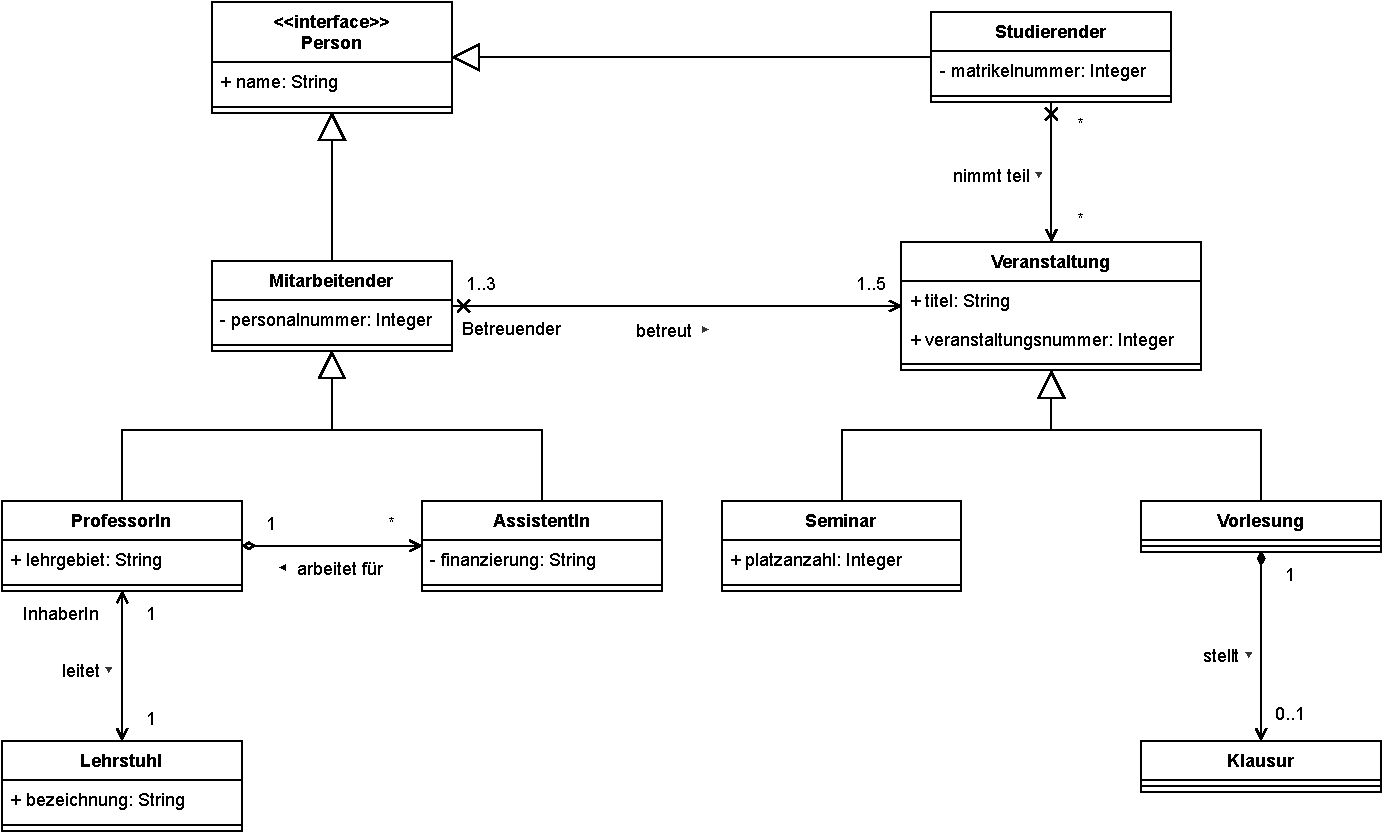
\includegraphics[width=\textwidth]{swt_wende_tim_h07_class_diagram.pdf}
        \caption{\texttt{class\_diagram}}
    \end{figure}

    \newpage    
    Finden Sie jeweils ein Beispiel, bei dem eine Aggregations- und eine Kompositionsbeziehung sinnvoll ist.
    Erläutern Sie kurz den Unterschied zwischen Aggretation und Komposition anhand des Bespiels.

    \begin{figure}[ht]
        \centering
        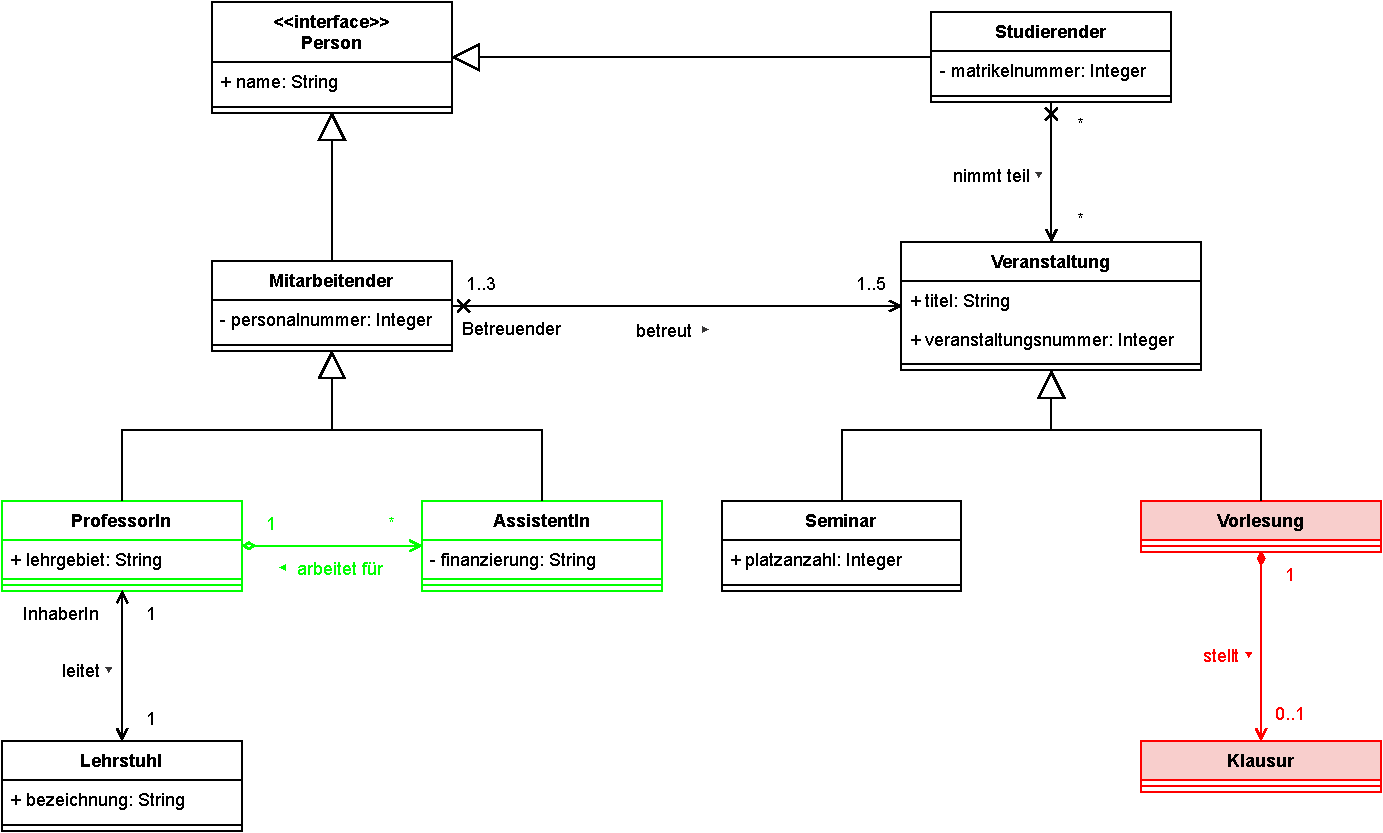
\includegraphics[width=0.75\textwidth]{swt_wende_tim_h07_class_diagram_diff.pdf}
        \caption{\texttt{class\_diagram\_diff}}
    \end{figure}

    Als Beispiel für die \textcolor{green}{Aggregation} habe ich die Beziehung zwischen \underline{ProfessorIn} und \underline{AssistentIn} gewählt.
    Im Gegensatz dazu steht die \textcolor{red}{Komposition}, welche durch die Beziehung zwischen \underline{Vorlesung} und \underline{Klausur} verkörpert wird.

    \vspace{1em}
    Einleitend fass \href{https://de.wikipedia.org/wiki/Assoziation_(UML)}{Wikipedia} es sehr gut zusammen (stark gekürzt):\\
    \textbf{Aggregation}:\\
    \gqq{Eine exakte Definition wird in der UML2 nicht gegeben [\ldots].
    Ein konkreter Nutzen lässt sich z. B. ableiten, indem man einem Ende einer Assoziation eine besondere Betonung zukommen lässt}\\
    \textbf{Komposition}:\\
    Der Unterschied zur Aggregation ist, dass ein Objekt, das als Ganzes Teile enthält, für die Existenz der Teile verantwortlich ist.

    Also anschaulich:
    \begin{figure}[ht]
        \centering
        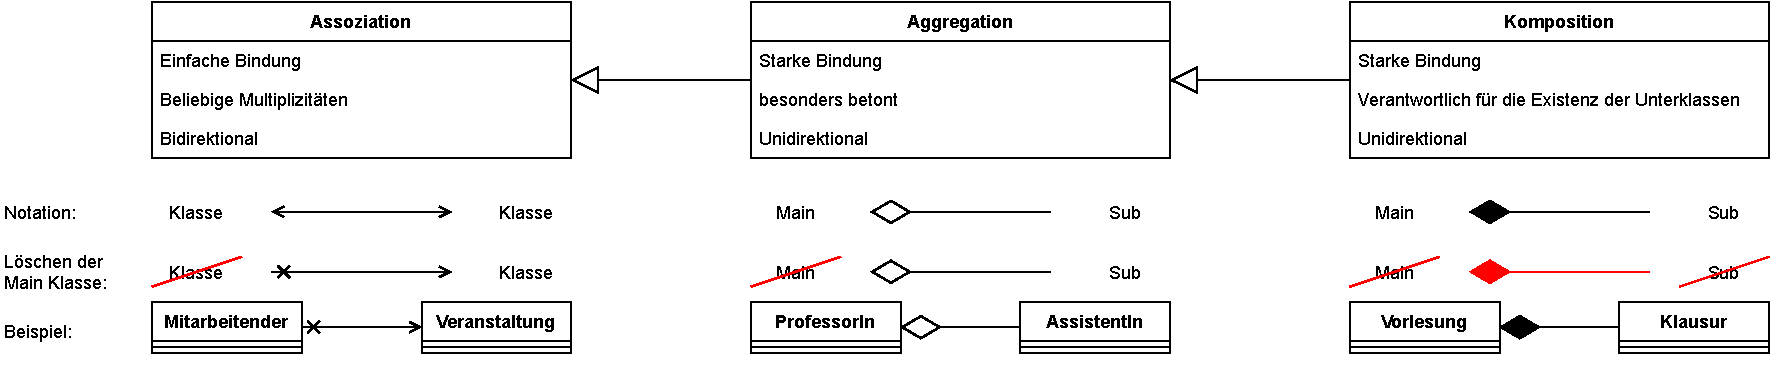
\includegraphics[width=0.75\textwidth]{swt_wende_tim_h07_class_diagram_chart.pdf}
        \caption{\texttt{class\_diagram\_chart}}
    \end{figure}

    Um diese Informationen auf unser Beispiel anzuwenden (bzg. der Klassen; nicht der Objekte):\\
    Ein/e \underline{AssistentIn} ist besonders *betont abhängig* von einem/einer \underline{ProfessorIn}.
    Diese Bindung ist beispielsweise stärker, als die Bindung eines \underline{Studierenden} zu einer \underline{Veranstaltung}, jedoch ist der/die \underline{ProfessorIn} nicht verantwortlich für die Existenz eines/einer \underline{AssistentIn}.\\
    Die \underline{Klausur} existiert jedoch ausschließlich, wenn die \underline{Vorlesung} existiert.
    Fällt diese Weg, wird das Objekt \underline{Klausur} automatisch entfernt.

    \vspace{1em}
    Anmerkungen zum Diagramm:
    \begin{itemize}
        \item Ich gehe davon aus, dass eine Klausur für nur eine Vorlesung genutzt werden kann.
            Da Dies nicht so genau aus der Aufgabenstellung erkennbar ist, sei dies hier erwähnt.
        \item Die Multiplizität am Pfeil \texttt{nimmt teil} bei \underline{Studierender} könnte auch mit Hilfe des Attributs \texttt{platzanzahl} aus \underline{Seminar} beschrieben werden.
            So könnte (um bei Java zu bleiben):\\
            \texttt{(Veranstaltung.isClass(Seminar)) ? ((Seminar) Veranstaltung).platzanzahl : *}\\
            die Genauigkeit der Obergrenze erhöhen.
    \end{itemize}

    \newpage
    \section*{Kohäsion und Kopplung}

    \begin{enumerate}
        \item Beschreiben Sie in eigenen Worten das Prinzip der Kohäsion und Kopplung in der Implementierung von Software-Projekten.

            Die Bindung verschiedener Objekte (Klassen/ Methoden/ ganzen Modulen/ \ldots), welche durch gegenseitige Methodenaufrufe oder Referenzen entsteht, wird Kopplung genannt.
            Die Dichte bzw. Anzahl dieser Bindungen wird durch das Maß der Kohäsion beschrieben.
            Dieses Maß beschreibt den logischen Zusammenhang der jeweiligen Kopplung.
            So geht das eine nie ohne das andere einher.
            Man möchte die paketintern Kohäsion der Bindung also so hoch wie möglich halten, und die Bindung der verschiedenen Pakete so gering wie möglich.
        
        \item Warum sind hohe Kohäsion und lose Kopplung der niedrigen Kohäsion und enger Kopplung vorzuziehen?
        
            Wenn man seinen Code in Pakete aufteilt, möchte man paketintern einen großen logischen Zusammenhang.
            Zusätzlich möchte man so wenige Querverbindungen zwischen den Paketen wie möglich erstellen, da man sonst in Gefahr läuft, dass jede Klasse in irgend einer Art und Weise abhänhig von einer Zweiten ist.
            Wenn man zusätzlich diese bereits reduzierten Querverbindungen auf eine Schnittstelle begrenzt, kann man \gqq{hinter} dieser \gqq{Proxy}-Klasse den Code beliebig ändern, ohne, dass man andere Klassen ebenfalls ändern muss.
            Die einzige Klasse, welche beeinflusst wird, ist die \gqq{Proxy}-Klasse. So hat man nur eine (ver-)Bindung und in den Paketen eine hohe Kohäsion.

        \item Geben Sie ein \textbf{eigenes} Beispiel in Form eines Klassendiagrammes für hohe Kohäsion und lose Kopplung an.
        
            \begin{figure}[ht]
                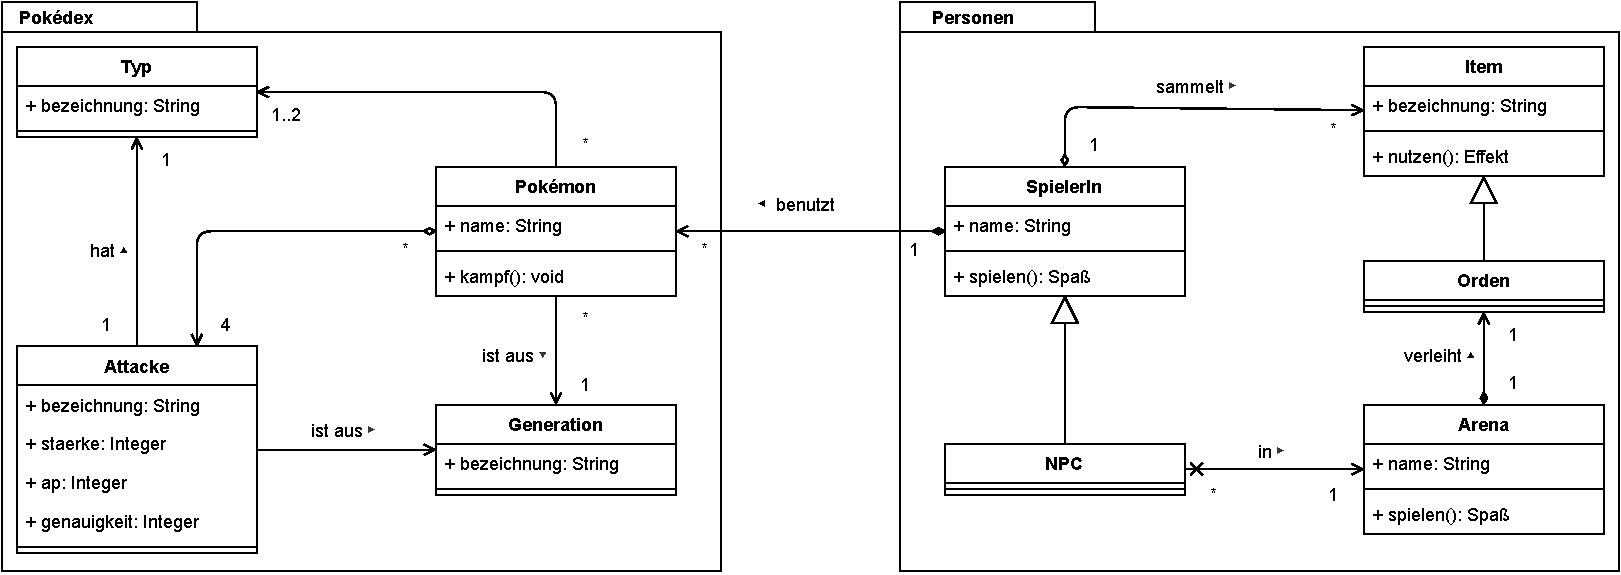
\includegraphics[width=\textwidth]{swt_wende_tim_h07_class_diagram_example.pdf}
                \caption{\texttt{class\_diagram\_example}}
            \end{figure}
    \end{enumerate}
\end{document}